\lecture{3}{}
\section{一维随机变量及其分布}%
\label{sec:一维随机变量及其分布}
\subsection{随机变量及其分布函数}%
\label{sub:随机变量及其分布函数}
\subsubsection*{随机变量}%
\label{subsub:随机变量}
\[
    \text{随机变量}
    \begin{cases}
        \text{函数}\\ 
        \text{连续}
    \end{cases}
.\] 
\begin{eg}
    下一个进入教室的同学可能是男是女,分别记为1,2,则有映射:
    \[
        \left\{ \text{男,女} \right\} \to \left\{ 1,2 \right\} 
    .\] 

    将离散的结果映射为坐标轴上离散的数值,所有的数值性的观测结果无需改变,如:下一个进入教室的同学身高为$\omega$,则有映射:
    \[
        X\left( \omega \right) =\omega
    .\] 
\end{eg}
\begin{defi}
    实值变量(无分布函数)使用小写字母,随机变量(有分布函数)使用大写字母

    对$\forall x\in \mathbb{R}$ ,$\left\{ X\le x \right\} =\left\{ \omega|X\left( \omega \right) \le x,\omega\le \Omega \right\}\in \mathscr{F} $,则$X$称为\textbf{概率空间的随机变量}
\end{defi}
\begin{eg}
    对于$\left\{ M,F \right\} \to \left\{ 1,2 \right\} $ ,取$x=1$ ,写出定义式:\[
        \left\{ X\le 1 \right\} =\left\{ M \right\} 
    .\] 

    同时由于$x\in \mathbb{R}$ ,取$x=1.5$时,$\left\{ X\le 1.5 \right\} =\left\{ M \right\} $
    取$x=4$时,$\left\{ X\le 4 \right\} =\left\{ M,F \right\} $
\end{eg}
由于$x\in \mathbb{R}$ ,则可以引入其他分布函数辅助,继而引用微积分理论

对于$\left( \Omega,\mathscr{F},P \right) $:\[
    P: \Omega\to \left[ 0,1 \right] 
.\] 
\begin{notation}
    $X$ 具有随机性(样本点具有随机性),是定义在$\Omega$ 上的函数

    $X$ 是随机变量时$\left\{ a\le X\le b \right\} ,a<b,a,b\in \mathbb{R}$ 均为随机事件

    $X$ 是随机变量,$g\left( x \right) $ 是非单点的实值函数,则$Y=g\left( X \right) $ 也是随机变量:\[
        Y\left( \omega \right) =g\left( X\left( \omega \right)  \right) 
    .\] 
\end{notation}
\begin{eg}
    对灯泡做寿命试验,用$X$ 表示测得灯泡的寿命,样本空间$\Omega=[0,+\infty)$,则:

    $A=$ “测得灯泡寿命大于500 h”$=\left\{ X>500 \right\} $

    $B=$ “测得灯泡寿命小于5000 h”$=\left\{ X\le 5000 \right\} $
\end{eg}
\subsubsection*{分布函数}%
\label{subsub:分布函数}
\begin{defi}
    分布函数:记\[
        F\left( x \right) =P\left\{ X\le x \right\} ,x\in \mathbb{R}
    .\]

    为$X$ 的分布函数
\end{defi}
\begin{eg}
    3白2黑,不放回取三次球,求取到的黑球个数$X$的分布函数

    $X$ 可以取到:0,1,2
    \[
        P\left\{ X=0 \right\} =\frac{\mathrm{C}_{3}^{3}}{\mathrm{C}_{5}^{3}},P\left\{ X=1 \right\} =\frac{\mathrm{C}_{2}^{1}\mathrm{C}_{3}^{2}}{\mathrm{C}_{5}^{3}},P\left\{ X=2 \right\} =\frac{\mathrm{C}_{2}^{2}\mathrm{C}_{3}^{1}}{\mathrm{C}_{5}^{3}}
    .\] 
    概率在坐标轴上体现:
    \begin{center}
        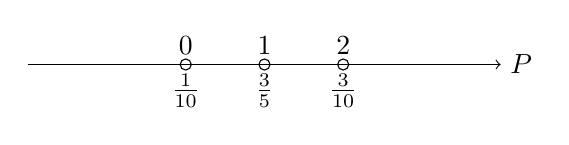
\begin{tikzpicture}
            \draw [->] (-2,0)--(4,0) node [right] {$P$};
            \draw [] (0,0) circle [radius=2pt] node [below] at(0,0) {$\frac{1}{10}$};
            \draw [] (1,0) circle [radius=2pt] node [below] at(1,0) {$\frac{3}{5}$};
            \draw [] (2,0) circle [radius=2pt] node [below] at(2,0) {$\frac{3}{10}$};
            \node [above] at(0,0) {$0$};
            \node [above] at(1,0) {$1$};
            \node [above] at(2,0) {$2$};
        \end{tikzpicture}
    \end{center}
    \[
        F\left( x \right) =P\left\{ X\le x \right\} =
        \begin{cases}
            0,x<0\\
            \frac{1}{10},x\in [0,1)\\
            \frac{1}{10}+\frac{3}{5}=\frac{7}{10},x\in [1,2)\\
            1,x\ge 2
        \end{cases}
    .\] 

    图像:
    \begin{center}
        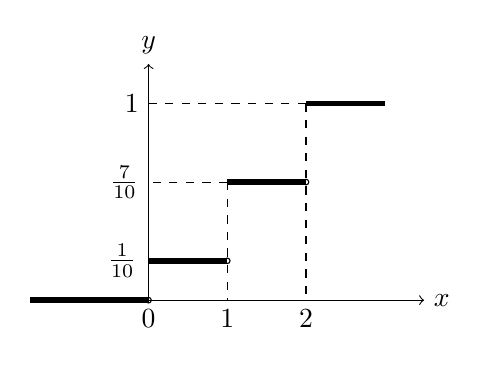
\begin{tikzpicture}[yscale=0.5,xscale=0.5]
            \node [below] at(0,0) {$0$};
            \draw [->] (-3,0)--(7,0) node [right] {$x$};
            \draw [->] (0,0)--(0,6) node [above] {$y$};
            \draw [dashed] (2,3)--(0,3) node [left] at(0,3) {${\frac{7}{10}}$};
            \draw [dashed] (4,5)--(0,5) node [left] at(0,5) {$1$};
            \draw [dashed] (2,3)--(2,0) node [below] at(2,0) {$1$};
            \draw [dashed] (4,5)--(4,0) node [below] at(4,0) {$2$};
            \draw [line width=2] (0,1)--(2,1) node [left] at(0,1) {${\frac{1}{10}}$};
            \draw [line width=2] (2,3)--(4,3);
            \draw [line width=2] (4,5)--(6,5);
            \draw [line width=2] (-3,0)--(0,0);
            \draw [] (2,1) circle [radius=2pt];
            \draw [] (4,3) circle [radius=2pt];
            \draw [] (0,0) circle [radius=2pt];
        \end{tikzpicture}
    \end{center}

\end{eg}
\begin{notation}
    分布函数的特性:

    1. 非负性:$P\in \left[ 0,1 \right] $

    2. 单调不减性

    3. 右连续性:\[
        F\left( x \right) =\lim_{t \to x+0^+} F\left( t \right) 
    .\] 

    3.1 不满足左连续,例:$P\left( 0 \right) -P\left( 0^- \right) \neq 0$

    4. 规范性:\[
        F\left( -\infty \right) =\lim_{x \to -\infty} F\left( x \right) =0,F\left( +\infty \right) =\lim_{x \to +\infty} F\left( x \right) =1
    .\] 
\end{notation}
关于$X$ 的事件都可以使用分布函数表示:
\[
    \begin{cases}
        P\left\{ X=a \right\} ={\lim_{\varepsilon \to 0^+}} P\left\{ a-\varepsilon<X\le a \right\} =F\left( a \right) -F\left( a-0^+ \right) \\
        P\left\{ a\le X<b \right\} =F\left( b-0^+ \right) -F\left( a-0^+ \right) \\
        \ldots\ldots
    \end{cases}
.\] 
\begin{eg}
    在$\left[ a,b \right] $ 内随机取一个数$X$ ,求$X$ 的分布函数

    关键区域:$x\in [a,b)$,\[
        \left\{ X\le x \right\} =\left\{ a\le X\le x \right\} 
    .\] 
    \[
        F\left( x \right) =P\left\{ X\le x \right\} =\frac{x-a}{b-a}
    .\] 
\end{eg}
作业:预习第2,3节
